This manuscript
(\href{https://SORTEE-Github-Hackathon.github.io/manuscript/v/540c54a0e1a9c1b107387aa297db8144b6a79d5e/}{permalink})
was automatically generated
from \href{https://github.com/SORTEE-Github-Hackathon/manuscript/tree/540c54a0e1a9c1b107387aa297db8144b6a79d5e}{SORTEE-Github-Hackathon/manuscript@540c54a}
on March 4, 2023.

\hypertarget{authors}{%
\subsection{Authors}\label{authors}}

\begin{itemize}
\item
  \textbf{Robert Crystal-Ornelas}
  
\includegraphics[width=0.16667in,height=0.16667in]{images/orcid.svg}
  \href{https://orcid.org/0000-0002-6339-1139}{0000-0002-6339-1139}
  · 
\includegraphics[width=0.16667in,height=0.16667in]{images/github.svg}
  \href{https://github.com/robcrystalornelas}{robcrystalornelas}
  · 
\includegraphics[width=0.16667in,height=0.16667in]{images/twitter.svg}
  \href{https://twitter.com/rob_c_ornelas}{rob\_c\_ornelas}
  Earth and Environmental Sciences Area, Lawrence Berkeley National Laboratory, Berkeley, CA 94720, USA
\item
  \textbf{Brandon P.M. Edwards}
  
\includegraphics[width=0.16667in,height=0.16667in]{images/orcid.svg}
  \href{https://orcid.org/0000-0003-0865-3076}{0000-0003-0865-3076}
  · 
\includegraphics[width=0.16667in,height=0.16667in]{images/github.svg}
  \href{https://github.com/BrandonEdwards}{BrandonEdwards}
  Department of Biology, Carleton University, Ottawa, ON K1S 5B6, Canada
\item
  \textbf{Katherine Hébert}
  
\includegraphics[width=0.16667in,height=0.16667in]{images/orcid.svg}
  \href{https://orcid.org/0000-0001-7866-6775}{0000-0001-7866-6775}
  · 
\includegraphics[width=0.16667in,height=0.16667in]{images/github.svg}
  \href{https://github.com/katherinehebert}{katherinehebert}
  · 
\includegraphics[width=0.16667in,height=0.16667in]{images/twitter.svg}
  \href{https://twitter.com/hebert_kat}{hebert\_kat}
  Département de biologie, Université de Sherbrooke, Québec, Canada
\item
  \textbf{Emma J. Hudgins}
  
\includegraphics[width=0.16667in,height=0.16667in]{images/orcid.svg}
  \href{https://orcid.org/0000-0002-8402-5111}{0000-0002-8402-5111}
  · 
\includegraphics[width=0.16667in,height=0.16667in]{images/github.svg}
  \href{https://github.com/emmajhudgins}{emmajhudgins}
  Department of Biology, Carleton University, Ottawa, ON K1S 5B6, Canada
\item
  \textbf{Luna L. Sánchez Reyes}
  
\includegraphics[width=0.16667in,height=0.16667in]{images/orcid.svg}
  \href{https://orcid.org/0000-0001-7668-2528}{0000-0001-7668-2528}
  · 
\includegraphics[width=0.16667in,height=0.16667in]{images/github.svg}
  \href{https://github.com/LunaSare}{LunaSare}
  · 
\includegraphics[width=0.16667in,height=0.16667in]{images/twitter.svg}
  \href{https://twitter.com/LunaSare}{LunaSare}
  School of Natural Sciences, University of California, Merced, USA
\item
  \textbf{Eric R. Scott}
  
\includegraphics[width=0.16667in,height=0.16667in]{images/orcid.svg}
  \href{https://orcid.org/0000-0002-7430-7879}{0000-0002-7430-7879}
  · 
\includegraphics[width=0.16667in,height=0.16667in]{images/github.svg}
  \href{https://github.com/Aariq}{Aariq}
  Communications \& Cyber Techologies, University of Arizona, Tucson, USA
\item
  \textbf{Matthew J. Grainger}
  
\includegraphics[width=0.16667in,height=0.16667in]{images/orcid.svg}
  \href{https://orcid.org/0000-0001-8426-6495}{0000-0001-8426-6495}
  · 
\includegraphics[width=0.16667in,height=0.16667in]{images/github.svg}
  \href{https://github.com/DrMattG}{DrMattG}
  · 
\includegraphics[width=0.16667in,height=0.16667in]{images/twitter.svg}
  \href{https://twitter.com/Ed_pheasant}{Ed\_pheasant}
  Terrestrial Biodiversity, Norwegian Institute for Nature Research - NINA, Postbox 5685 Torgarden, 7485 Trondheim, Norway
\item
  \textbf{Vivienne Foroughirad}
  
\includegraphics[width=0.16667in,height=0.16667in]{images/orcid.svg}
  \href{https://orcid.org/0000-0002-8656-7440}{0000-0002-8656-7440}
  · 
\includegraphics[width=0.16667in,height=0.16667in]{images/github.svg}
  \href{https://github.com/vjf2}{vjf2}
  · 
\includegraphics[width=0.16667in,height=0.16667in]{images/twitter.svg}
  \href{https://twitter.com/vforoughirad}{vforoughirad}
  Department of Biology, Georgetown University, Washington, DC, USA
\item
  \textbf{Allison D. Binley}
  
\includegraphics[width=0.16667in,height=0.16667in]{images/orcid.svg}
  \href{https://orcid.org/0000-0001-8790-9935}{0000-0001-8790-9935}
  · 
\includegraphics[width=0.16667in,height=0.16667in]{images/github.svg}
  \href{https://github.com/adbinley}{adbinley}
  · 
\includegraphics[width=0.16667in,height=0.16667in]{images/twitter.svg}
  \href{https://twitter.com/AllisonBinley}{AllisonBinley}
  Department of Biology, Carleton University, Ottawa, ON K1S 5B6, Canada
\item
  \textbf{Cole B. Brookson}
  
\includegraphics[width=0.16667in,height=0.16667in]{images/orcid.svg}
  \href{https://orcid.org/0000-0003-1237-4096}{0000-0003-1237-4096}
  · 
\includegraphics[width=0.16667in,height=0.16667in]{images/github.svg}
  \href{https://github.com/colebrookson}{colebrookson}
  Department of Biological Sciences, University of Alberta, Edmonton, AB, Canada
\item
  \textbf{Kaitlyn M. Gaynor}
  
\includegraphics[width=0.16667in,height=0.16667in]{images/orcid.svg}
  \href{https://orcid.org/0000-0002-5747-0543}{0000-0002-5747-0543}
  · 
\includegraphics[width=0.16667in,height=0.16667in]{images/github.svg}
  \href{https://github.com/kaitlyngaynor}{kaitlyngaynor}
  · 
\includegraphics[width=0.16667in,height=0.16667in]{images/twitter.svg}
  \href{https://twitter.com/kaitlyngaynor}{kaitlyngaynor}
  Departments of Zoology and Botany, University of British Columbia, Vancouver, BC, Canada
\item
  \textbf{Saeed Shafiei Sabet}
  
\includegraphics[width=0.16667in,height=0.16667in]{images/orcid.svg}
  \href{https://orcid.org/0000-0001-5919-2527}{0000-0001-5919-2527}
  · 
\includegraphics[width=0.16667in,height=0.16667in]{images/github.svg}
  \href{https://github.com/shafieisabets}{shafieisabets}
  · 
\includegraphics[width=0.16667in,height=0.16667in]{images/twitter.svg}
  \href{https://twitter.com/SaeedSHSABET}{SaeedSHSABET}
  Fisheries Department, Faculty of Natural Resources, University of Guilan, Sowmeh Sara, Iran
\item
  \textbf{Ali Güncan}
  
\includegraphics[width=0.16667in,height=0.16667in]{images/orcid.svg}
  \href{https://orcid.org/0000-0003-1765-648X}{0000-0003-1765-648X}
  · 
\includegraphics[width=0.16667in,height=0.16667in]{images/github.svg}
  \href{https://github.com/Aguncan}{Aguncan}
  · 
\includegraphics[width=0.16667in,height=0.16667in]{images/twitter.svg}
  \href{https://twitter.com/aliguncan}{aliguncan}
  Department of Plant Protection, Faculty of Agriculture, Ordu University, 52200, Ordu, Turkey
\item
  \textbf{Friederike Hillemann}
  
\includegraphics[width=0.16667in,height=0.16667in]{images/orcid.svg}
  \href{https://orcid.org/0000-0002-8992-0676}{0000-0002-8992-0676}
  · 
\includegraphics[width=0.16667in,height=0.16667in]{images/github.svg}
  \href{https://github.com/fhillemann}{fhillemann}
  Department of Human Behavior, Ecology and Culture, Max Planck Institute for Evolutionary Anthropology, Leipzig, Germany
\item
  \textbf{Helen Weierbach}
  
\includegraphics[width=0.16667in,height=0.16667in]{images/orcid.svg}
  \href{https://orcid.org/0000-0001-6348-9120}{0000-0001-6348-9120}
  · 
\includegraphics[width=0.16667in,height=0.16667in]{images/github.svg}
  \href{https://github.com/helenweierbach}{helenweierbach}
  · 
\includegraphics[width=0.16667in,height=0.16667in]{images/twitter.svg}
  \href{https://twitter.com/HWeierbach}{HWeierbach}
  Earth and Environmental Sciences Area, Lawrence Berkeley National Laboratory, Berkeley, CA 94720, USA
\item
  \textbf{Dylan G. E. Gomes}
  
\includegraphics[width=0.16667in,height=0.16667in]{images/orcid.svg}
  \href{https://orcid.org/0000-0002-2642-3728}{0000-0002-2642-3728}
  · 
\includegraphics[width=0.16667in,height=0.16667in]{images/github.svg}
  \href{https://github.com/dylangomes}{dylangomes}
  (Current) National Academy of Sciences NRC Research Associateship Program, Northwest Fisheries Science Center, National Marine Fisheries Service, National Oceanic and Atmospheric Administration, Seattle, WA, USA 98112; (Former) Cooperative Institute for Marine Resources Studies, Hatfield Marine Science Center, Oregon State University, Newport, OR, USA 97365
\item
  \textbf{Pedro Henrique Pereira Braga}
  
\includegraphics[width=0.16667in,height=0.16667in]{images/orcid.svg}
  \href{https://orcid.org/0000-0002-1308-1562}{0000-0002-1308-1562}
  · 
\includegraphics[width=0.16667in,height=0.16667in]{images/github.svg}
  \href{https://github.com/pedrohbraga}{pedrohbraga}
  · 
\includegraphics[width=0.16667in,height=0.16667in]{images/twitter.svg}
  \href{https://twitter.com/pedrohp_braga}{pedrohp\_braga}
  Department of Biology, Concordia University, 7141 Sherbrooke Street West, Montreal, QC H4B 1R6, Canada
\end{itemize}

\hypertarget{abstract}{%
\subsection{Abstract}\label{abstract}}

Researchers in ecology and evolutionary biology are increasingly dependent on computational code to conduct research. Hence, the use of efficient methods to share, reproduce, and collaborate on code as well as document research is fundamental.
GitHub is an online, cloud-based service that can help researchers track, organize, discuss, share, and collaborate on software and other materials related to research production, including data, code for analyses, and protocols.

Despite these benefits, the use of GitHub in ecology and evolution is not widespread.
To help researchers in ecology and evolution adopt useful features from GitHub to improve their research workflows, we review twelve practical ways to use the platform.
We outline features ranging from low to high technical difficulty: storing code, managing projects, coding collaboratively, conducting peer review, and writing a manuscript.
Given that members of a research team may have different technical skills and responsibilities, we describe how the optimal use of GitHub features may vary among members of a research collaboration.
As more ecologists and evolutionary biologists establish their workflows using GitHub, the field can continue to push the boundaries of collaborative, transparent, and open research.

\hypertarget{introduction}{%
\subsection{Introduction}\label{introduction}}

Most scientists, including ecologists and evolutionary biologists, depend on computational tools for their research (\protect\hyperlink{ref-fJWFe93e}{Hannay et al., 2009}).
Researchers write and use software packages or write code (hereafter, code) to perform scientific tasks ranging from data management, data analysis, and study replication, to the application and the development of tools for hypothesis testing.
Maintaining code for scientific collaboration requires an efficient and well-documented work-flow (\protect\hyperlink{ref-1Kqna6l2}{J. M. Perkel, 2020}).
To facilitate this process, scientists have been adopting tools from information and systems technology, such as cloud-based services for documentation and version control {[}\emph{e.g.}, the Google Suite, the Microsoft Suite, DropBox, and GitHub (\protect\hyperlink{ref-10ghgV3S8}{J. Perkel, 2016}){]}.
Within the spectrum of cloud-based services for collaboration, GitHub is uniquely positioned (\protect\hyperlink{tbl:compare}{Table 1}) to benefit scientists because it is designed to store, track changes, and enable collaboration on computer code---fundamental components of modern research.
Albeit, most researchers lack exposure to adequate programming and coding practices and thus dedicate valuable time and effort to self-teaching research-facilitating tools.
GitHub is one of the most used web-based platforms for computational version control and collaboration, and in this paper, we provide researchers in ecology and evolutionary biology (EEB) with practical workflows to use GitHub to facilitate their collaborative research and code management practices.

GitHub (\url{https://github.com}) provides a simple but powerful web interface that allows users to participate in projects by contributing, modifying and discussing existing code, reporting bugs, discovering code and data, and publishing new code.
Github allows users to store files and directories in repositories, and keeps a chronological record of modifications (\protect\hyperlink{ref-RVetqmsg}{Bryan, 2018}) (see \protect\hyperlink{definitions}{Box 1}).
Beyond storage and record-tracking, file management in GitHub is integrated with several communication features, allowing users to engage in discussions, to plan and collaborate in code, and publish information to a webpage (Github Issues, Github Discussions, Github Pages; see \protect\hyperlink{definitions}{Box 1}).
These features contrast with traditional practices of directly sharing files through email, other cloud-based services or physical storage units, which become challenging and time-consuming in long-term and collaborative projects (\protect\hyperlink{ref-4ny1onB0}{Ram, 2013}).
By allowing users to easily integrate versioning, communication, collaboration with research code and data, Github paves the way for easier implementation of open science practices within research projects (\protect\hyperlink{ref-kEX5dgzK}{Perez-Riverol et al., 2016}).

Git is the version control system that enables the collaborative tools available on GitHub.
Git was originally developed as a fast, lightweight and open-source system to allow software engineers to efficiently develop and collaborate in projects (\protect\hyperlink{ref-1CM2EcdVk}{\emph{Git - A Short History of Git}, n.d.}).
Since its launch in 2005, Git has become the leading version control system in software development and in other disciplines that require collaboration and community contributions, such as in scientific research (\protect\hyperlink{ref-7q3wZN6d}{Spinellis, 2012}).
Knowledge of basic concepts of Git (such as commit, push, pull, and checkout; see \protect\hyperlink{definitions}{Box 1}) is recommended to understand how GitHub keeps track of changes to files and folders.
Nevertheless, the GitHub web-based platform and its integrated development environments (such as GitHub Desktop) allow users to perform most repository and data management operations without using the command console, making these functionalities available to users who are less familiar with software development.

Version control involves tracking the state of the files and directories which are stored in a ``repository'' (see \protect\hyperlink{definitions}{Box 1}).
A basic workflow using Git and GitHub is to: (i) create a remote repository that is synchronized with files and directories stored locally; (ii) modify these files, either locally or remotely; (iii) frequently ``commit'' (or record) changes to these files (see \protect\hyperlink{definitions}{Box 1}) along with a description of modifications; (iv) synchronize commits with GitHub (see ``push'' and ``pull'' in \protect\hyperlink{definitions}{Box 1}) so that the repository on the web and the local repositories are up-to-date.
Repositories, which contain files, their modifications, and the description of their changes can then be accessed by chosen collaborators or, whenever applicable, the public, who can easily download and synchronize them to their own computers (see ``clone'' in \protect\hyperlink{definitions}{Box 1}).
Commits act like snapshots, one can view or even revert the state of the project to any previous commit.
If the modified files are plain text, only the differences from the previous commit are recorded, allowing you to frequently commit changes without causing the size of the project to grow excessively.
This provides a safe and less cluttered alternative to frequently making full copies of documents at different points in their evolution (\emph{e.g.} \texttt{analysis.R}, \texttt{analysis\_v2.R}, \texttt{analysis\_FINAL.R}).
While focusing on technical details about the use of Git and GitHub is beyond the scope of this study, we recommend users explore available resources to become more familiar with version control features (see Perez-Riverol et al. (\protect\hyperlink{ref-kEX5dgzK}{2016}), Blischak et al. (\protect\hyperlink{ref-PlcxShQU}{2016}), and Kalliamvakou et al. (\protect\hyperlink{ref-ndfO9H}{2015})).

The expansive GitHub user-community and numerous GitHub resources have boosted its popularity {[}Perez-Riverol et al. (\protect\hyperlink{ref-kEX5dgzK}{2016}); Bryan (\protect\hyperlink{ref-RVetqmsg}{2018}); \url{https://happygitwithr.com}; \url{https://ourcodingclub.github.io}{]}.
Nevertheless, although multiple articles have encouraged researchers in EEB to adopt GitHub as part of their research process (\protect\hyperlink{ref-3DKwn1sY}{Lowndes et al., 2017}; \protect\hyperlink{ref-10ghgV3S8}{J. Perkel, 2016}), its use is still not widespread.
First-time users without formal training in information technology may face steep learning curves because GitHub and its features have been centered on software development (\protect\hyperlink{ref-139b0pSGc}{Leibzon, 2016}).
Moreover, domain-specific resources providing tractable examples and practical guidance for researchers in EEB on GitHub are scarce {[}but see Kim et al. (\protect\hyperlink{ref-lJAgyhYq}{2022}); \url{https://ourcodingclub.github.io}; \url{https://www.openscapes.org}{]}.
Widespread adoption of GitHub for collaborating on research tasks can ultimately enable EEB researchers to spend less time on creating novel processes for collaboration and more time on their research (\protect\hyperlink{ref-ydrk01SR}{Briney et al., 2020}).
More importantly, expanding the availability of data and code management standards---of which GitHub is one increasingly important component---makes research more reproducible and collaborative (\protect\hyperlink{ref-13QX8XU3J}{Alston \& Rick, 2021}; \protect\hyperlink{ref-VDJput1V}{Gomes et al., 2022}).

This paper is the result of an academic hackathon held during the 2021 conference for the Society for Open, Reliable, and Transparent Ecology and Evolutionary Biology (SORTEE, \url{https://www.sortee.org}).
We convened around thirty researchers in EEB with varying levels of familiarity with the usage of GitHub in research projects to showcase and discuss how existing features can contribute to documentation and collaboration in EEB research.
During the hackathon, we identified the need for formal discussions on how EEB researchers can benefit from GitHub and its features.
Here, we outline twelve practical ways that EEB researchers can use GitHub features for more collaborative, transparent, and reproducible science.
We also provide critical perspectives on features that could be improved and catered towards research development.

\hypertarget{definitions}{%
\subsubsection{Box 1}\label{definitions}}

\begin{tablenos:no-prefix-table-caption}

\begin{longtable}[]{@{}
  >{\raggedright\arraybackslash}p{(\columnwidth - 0\tabcolsep) * \real{1.0000}}@{}}
\toprule
\begin{minipage}[b]{\linewidth}\raggedright
Glossary
\end{minipage} \\
\midrule
\endhead
\textbf{repository}: A repository (commonly shortened to ``repo'') is a collection of files (\emph{e.g.}, a directory) tracked by Git. Repositories are managed by an owner and can be made either ``public'', to be visible to all GitHub users, or ``private'', to selected owner-specified users. Repositories can be either ``local'' and saved on an individual's computer or ``remote'' and stored on the cloud via GitHub's web platform. \\
\textbf{fork}: A fork is a copy of a \textbf{repository} hosted on GitHub. If a repository is public, then anyone can make a fork. Even if they do not have access to \textbf{push} to the original repository, they can make a fork and edit it independently. Forks are linked to the original GitHub repository and ``upstream'' changes (\emph{i.e.}, those in the original repository) can be \textbf{merged} to keep the fork up-to-date with the original project. Changes made in the fork can be integrated into the original project via \textbf{pull requests}. \\
\textbf{clone}: Cloning a \textbf{repository} is a way of making a local copy (\emph{i.e.}, on your computer) of a GitHub \textbf{repository}. If you have access to \textbf{push} to a \textbf{repository}, this can be a first step to contributing to a project. \\
\textbf{branch}: Git workflow timelines or repositories are analogous to trees, with a main working project and diverging branches that are pointers to changes during the development process. A git branch is an alternative line of development for a project (repository). Branches allow users to add new features or modifications to the project without affecting the main part of the project. Development branches can be created at any point in time and work on each branch can continue independently. Branching is useful for testing out new ideas (both code and text) which may or may not eventually get integrated into the main branch of the project. Branches can also be used to isolate contributions of multiple contributors. Each person working on their own branch eliminates problems that may arise if conflicting edits are \textbf{pushed} to the same remote branch. Changes in a development branch can be \textbf{merged} into the main branch via \textbf{pull requests}. Branches can only be made by those who are given access to the project \textbf{repository}. \\
\textbf{commit}: Commits are snapshots of the development of a project. In Git, versions of files and directories are uniquely identified as ``commits'', allowing one to identify and track modifications line-by-line. Commits can include changes in multiple files and must include a brief commit message describing the changes made. A typical workflow is to make some related changes in files, add a commit message (\emph{e.g.}, ``Generate and include results figure''), and after several commits \textbf{push} those commits to the remote (\emph{i.e.}, cloud-based) GitHub \textbf{repository}. \\
\textbf{push and pull}: When \textbf{commits} are made in a project locally, they must be synced with the remote GitHub repository by \textbf{pushing} them. Changes on a GitHub repository can then be \textbf{pulled} to keep your local version of the project up-to-date with the remote. \\
\textbf{pull request}: A pull request is a request for changes made on an individual's \textbf{branch} in the repository or in a user's \textbf{fork} to be merged to the repository. Pull requests contain a description of the changes alongside all code required for testing and review by other users prior to being merged into the repository. \\
\textbf{merge}: Combining \textbf{commits} from two different branches together into one \textbf{branch}. \\
\textbf{release}: At any point a release can be made on GitHub to mark a significant milestone in the progression of a \textbf{repository}. While this GitHub feature is designed with releases of new versions of code in mind (\emph{e.g.}, v1.0.0), it can also be used to create a snapshot of a repository at significant stages like pre-print, submission, revision, and acceptance of an associated manuscript. \\
\textbf{community}: A forum where GitHub users can ask for advice, offer solutions to questions, and share ideas (\url{https://github.community/}). \\
\bottomrule
\end{longtable}

\end{tablenos:no-prefix-table-caption}

\hypertarget{twelve-practical-ways-github-can-accelerate-research-in-ecology-and-evolution}{%
\subsection{Twelve practical ways GitHub can accelerate research in ecology and evolution}\label{twelve-practical-ways-github-can-accelerate-research-in-ecology-and-evolution}}

\hypertarget{storing-sharing}{%
\subsubsection{Storing and sharing research compendia}\label{storing-sharing}}

An EEB research compendium includes all computational materials related to research production, including data, code for analyses and protocols.
Safely storing these files is essential to protect against accidental modifications or deletions.
Many researchers begin using GitHub to backup their research compendium (\protect\hyperlink{ref-MwwMapRG}{Marwick et al., 2018}) into a centralized, readily-available remote server (see \protect\hyperlink{definitions}{Box 1}).
This practice has the advantages of facilitating collaboration, integrating data and code archiving, allowing file versions to be accessed and restored, and further contributing to open science practices (\protect\hyperlink{ref-gLby7jt1}{Borghi \& Van Gulick, 2022}).
Changes made to files in version-controlled repositories are accompanied by authored descriptions of modifications (\protect\hyperlink{definitions}{Box 1}).
Later, the entire history of commits and their commit messages are viewable and can be audited similarly to physical laboratory notebooks (\protect\hyperlink{ref-4ny1onB0}{Ram, 2013}).
GitHub allows administrative control over who can view and modify repositories, and the process of cloning, forking and suggesting changes through pull requests (see \protect\hyperlink{definitions}{Box 1}) ensures code owners have full control over code and documents.
Repositories can be changed from public to private, allowing data storage and management without sacrificing the privacy that may be necessary for certain compendia.
With this, researchers can grant collaborators read and/or write access to files in private repositories to pursue pre-publication analyses or writing in privacy.

GitHub limits committed file sizes to 100 Mb (megabytes) (\protect\hyperlink{ref-1Co6ZZjF1}{\emph{About Large Files on GitHub}, n.d.}), which may require external file storage alternatives (such as local or cloud-hosting) for some parts of research compendia.
However, users can still track versions of remotely- or locally-stored files in their repositories using Git Large File Storage (\url{https://git-lfs.github.com}).

\hypertarget{project-continuity}{%
\subsubsection{Project continuity}\label{project-continuity}}

Projects in ecology and evolution often involve research professionals holding limited-term positions, such as graduate students, research assistants, and post-doctoral fellows (\protect\hyperlink{ref-D4C4k4ak}{Fehr et al., 2021}).
Without clear plans on project continuity, research code and data management upkeep tends to fall off as researchers move on to new projects or other institutions.
Additionally, code and data can be difficult to access and recover when kept only on personal devices (\protect\hyperlink{ref-19kmNxiHc}{Vines et al., 2014}).

GitHub can facilitate project continuity in research by making code and data handover between users easier (\protect\hyperlink{ref-D4C4k4ak}{Fehr et al., 2021}; \protect\hyperlink{ref-4ny1onB0}{Ram, 2013}).
Through version control, the history of code and data from projects in ecology and evolution becomes accessible to future laboratory members and collaborators (\protect\hyperlink{ref-3DKwn1sY}{Lowndes et al., 2017}).
Repositories and organizations can have designated data and code owners {[}or more appropriately, ``data stewards''; see Hampton et al. (\protect\hyperlink{ref-iIEKCTLU}{2015}), \emph{About Code Owners} (\protect\hyperlink{ref-s91uGRZ2}{n.d.}){]}, who can also change through time, allowing for the transition of code between research cohorts (see also \protect\hyperlink{organizations}{``Organizing and managing teams''}).
Other project collaborators can contribute to repository design and development, and their active involvement can both aid authors ability to act as guarantors, and the clarity and reproducibility of the project for future users.
In (Figure \ref{fig:github-diagram}), we highlight several elements of recommended repository structure, and the various ways that contributors may interact with them.

Software compatibility during the analysis and reanalysis of project data can be ensured by storing information about software dependencies and their versions within the same project repository.
With more advanced practices, one can remotely install and execute scripts using specific versions of software within GitHub's project automation tools, GitHub Actions (see below).

In addition to projects, long-term management of laboratory materials (such as notebooks or experimental protocols) can also be done within GitHub, a practice that has been increasingly adopted across many fields (\protect\hyperlink{ref-10ghgV3S8}{J. Perkel, 2016}), including applied ecology (\emph{e.g.}, \url{https://scheuerell-lab.github.io/lab-book}), biogeography and global change biology (\emph{e.g.}, \url{https://github.com/HuckleyLab/how_we_work}), and microbial ecology (\emph{e.g.}, \url{https://github.com/CarBBAS/uqam-guide}).

\hypertarget{project-management}{%
\subsubsection{Project management}\label{project-management}}

Modern research in ecology and evolution is highly collaborative, bringing together multidisciplinary teams from various institutions (\protect\hyperlink{ref-1HhzKAC1K}{Goring et al., 2014}).
On GitHub, collaborators can share feedback, brainstorm ideas, and troubleshoot problems (Figure \ref{fig:github-diagram}).
Project management can happen via three GitHub repository features: ``Issues'', ``Discussion'' and ``Projects'' (\protect\hyperlink{definitions}{Box 1}).
Github Issues allow for discrete tasks and sub-tasks to be identified, assigned to team members, and categorized with custom labels.
Github Discussions serve as a message board for conversation.
Finally, GitHub Projects provides users with real-time tracking of project priorities and status (\protect\hyperlink{ref-RhBKe0MG}{\emph{About Projects}, n.d.}).
For instance, one can create a discussion on a project repository to decide which method to apply for biodiversity data analysis.
Then, an issue can be created to establish steps and responsibilities including data formatting, statistical analyses, figure generation, and issue resolution (\protect\hyperlink{ref-3UAritXO}{\emph{Issues · Fmsabatini/sPlotOpen\_Manuscript}, n.d.}, =is\%3Aissue+is\%3Aclosed; \emph{e.g.}, see issues and discussions in the sPlotOpen manuscript repository, \protect\hyperlink{ref-doi:10.1111ux2fgeb.13346}{\textbf{doi:10.1111/geb.13346?}}).
Using GitHub for all project-related conversation and planning, rather than email or messaging tools, makes it easier to keep track of progress throughout the lifespan of a project.
However, one can opt to receive new issues, discussions, and responses as emails and can post replies by email as well.\\
This allows for centralized communication for a team even when some members prefer to use email for communication.
Unlike emails and messages which can get lost as more new tasks arise, GitHub issues are intentionally closed by repository administrators hiding the issue from view (closed issues remain accessible but not immediately visible).

\hypertarget{educational-materials}{%
\subsubsection{Educational materials}\label{educational-materials}}

GitHub supports a broad set of mechanisms for hosting educational materials.
The entire process of running a course, workshop, or lecture, can all be done openly on GitHub including material development, web hosting, and delivery, and even submission and grading of assignments.
While there are other purpose-built platforms for this, GitHub provides a free, open-source alternative.

Syllabi, presentations, and other course materials can be version-controlled, stored and managed in GitHub.
While any file type for presentations and documents can be stored and tracked in repositories, GitHub can directly render and display certain markup languages, such as HyperText Markup Language (HTML) and Markdown documents, making these file types especially useful for educational materials.
Course content can then be delivered to the audience by sharing links of web-hosted GitHub Pages (see \protect\hyperlink{hosting-a-website}{Hosting a Website}), GitHub Repositories and/or GitHub Organizations.
Finally, instructors can host and assign student work to be submitted collaboratively or individually as code and text files, and even build autograding tests using the GitHub Classroom tool (\url{https://classroom.github.com}).

Although time-consuming, adopting these features in classrooms can integrate the learning of version-control and GitHub practices with the learning of course contents, and thus boost students' feelings of self-efficacy and confidence (\protect\hyperlink{ref-dqrFjoSb}{Trujillo \& Tanner, 2014}).

\hypertarget{hosting-a-website}{%
\subsubsection{Hosting a website}\label{hosting-a-website}}

Personal or laboratory websites can improve the sharing of research findings, build online presence, and increase coordination of research efforts (\protect\hyperlink{ref-HiIPSSHV}{Smaglik, 2007}).
Despite researchers in ecology and evolution generally lacking experience in building or hosting webpages, many tools have been developed to help this process.
Static websites can now be easily built {[}using, for example Quarto (\url{https://quarto.org}), RMarkdown, Hugo (\url{https://gohugo.io}), GitHub Website templates (\url{https://github.com/topics/website-template})), stored in a repository, and be readily hosted by activating GitHub's Pages (\url{https://pages.github.com}) feature.
Creating and hosting websites on GitHub Pages is more complex than out-of-the-box platforms (\emph{e.g.}, Wix, Weebly, Google Sites).
However, free hosting, widely available template customization, and versioning are strong advantages over alternatives.{]}.
Users can set up workflows associated with their repositories that are triggered by events (\emph{e.g.}, push, pull request or at specified times) for remote servers to perform user-specified steps and actions.
These actions are highly configurable and have numerous applications, such as automatically running analyses and creating figures when data or code are updated, incorporating changes to websites or applications, testing modifications to software (\emph{e.g.}, R or Python libraries).
Action workflows can be found in GitHub's Marketplace (\url{https://github.com/marketplace?type=actions}) or, alternatively, in open user repositories.

\hypertarget{organizations}{%
\subsubsection{Organizing and managing teams}\label{organizations}}

GitHub Organizations are shared virtual spaces that allow teams to work in different repositories, while remaining tied together under a larger group, such as a laboratory, department, or project involving several teams.
Organizations allow larger projects with many steps or moving parts to be constrained to one virtual space, where outputs and sub-projects can be easily accessed and located without relying on individuals.
Because the repositories are grouped, members can reference and contribute to each other's work without necessarily being part of the same repository, broadening the accessibility and longevity of code and writing contributions.

Contributors can be assembled into teams within an organization, which allows administrators to assign roles, tasks, and repository modification permissions to organization members.
Whereas access to repositories is usually assigned to individual contributors, Organizations facilitate the management of access permissions by allowing teams to be granted access to specific repositories.
This ensures repositories with sensitive information remain as restricted as needed, while others stay open and accessible to selected member groups.
The organization structure also allows for issue tracking and discussions related to research content and progress.

As an example, GitHub Organizations are particularly well-suited to host documents and projects within a laboratory, such as research compendia, codes of conduct, protocols, training documents, and other relevant documents that evolve collaboratively over time.
In this way, teams have full ownership of repositories within an organization, while ensuring that these materials stay accessible to the laboratory after people have moved on or when locally-stored data are lost.
This application extends to research centres, which may include several distinct projects that remain linked to institutions {[}\emph{e.g.}, the German Centre for Integrative Biodiversity Research (iDiv, \url{https://github.com/idiv-biodiversity}){]}.
The team organizing the hackathon which inspired this article used a GitHub Organization (SORTEE-Github-Hackathon, \url{https://github.com/SORTEE-Github-Hackathon}) to centralize the project development, from meeting notes to, ultimately, this manuscript.
Organizations are also convenient for hosting learning materials, including lectures or workshops, such as the Québec Centre for Biodiversity Science R Workshop Series (QCBSRworkshops, \url{https://github.com/QCBSRworkshops}) or the University of Edinburgh's Coding Club (Coding Club, \url{https://github.com/ourcodingclub}), which may be continuously updated by an ever-evolving group of contributors.

\hypertarget{discussion}{%
\subsection{Discussion}\label{discussion}}

\hypertarget{the-promise-of-github-for-eeb-researchers}{%
\subsubsection{The promise of GitHub for EEB researchers}\label{the-promise-of-github-for-eeb-researchers}}

There have been many calls for researchers outside of the software development community to adopt GitHub for their collaborative research (\protect\hyperlink{ref-UsTxAq4f}{Anbaroğlu, 2021}; \protect\hyperlink{ref-1Du6fzB8g}{Crystal‐Ornelas et al., 2021}; \protect\hyperlink{ref-10ghgV3S8}{J. Perkel, 2016}).
These calls come in light of the continuous shift towards open-science and the increasing computational and data requirements in EEB.
While tools like the Google Suite and DropBox enable rapid sharing and collaboration of some research documents, GitHub brings together features that directly integrate open science practices, such as the association of public discussions with data, code and findings, tracking multiple rounds of edits to files in a sensible way for easy review, and managing complex research projects with many collaborators and goals.
Until now, resources and practical guidance on using GitHub within the EEB community have been dispersed across blog posts, as well as written and video tutorials (\protect\hyperlink{tips}{Box 2}).
These resources have been useful for learning to use GitHub in our own research, as ecologists and evolutionary biologists.
We expect that situating the main uses of GitHub in EEB alongside examples in this paper will be useful to the EEB community.

The twelve use cases we described here can leverage GitHub to enable more transparent and collaborative research in ecology and evolution (Figure \ref{fig:scatterblob}).
Most of these uses can be quickly integrated into the research practices of users (\emph{e.g.}, storing data, creating virtual notebooks, making code citable).
Making stored data and code citable usually involves creating a repository on GitHub, pushing code and data, and then integrating a DOI minting service to the repository (\emph{e.g.}, with Zenodo or OSF; see below).
On the other hand, some cases we described here, including course material development, web hosting, and automation, require greater effort and time commitment, but have the potential to make EEB research more open, accessible, and collaborative.
Managing full research projects or laboratories on GitHub require careful thought as to how to delegate tasks, such as reviewing pull requests or creating issues.
For example, collaboratively authoring a paper using GitHub, as we have done here, involves a learning curve for co-authors less familiar with the intricacies of GitHub, requires overhead to set up automation frameworks through GitHub Actions, and especially, the commitment from all co-authors to use GitHub when modifying and reviewing the text.
Despite the potential applications of GitHub to EEB research, we acknowledge that researchers might still look to other platforms for research collaboration.

\hypertarget{other-platforms-for-collaboration}{%
\subsubsection{Other platforms for collaboration}\label{other-platforms-for-collaboration}}

Despite its strong collaborative potential, we describe two use cases where GitHub falls short of highly collaborative work.

First, real-time document editing is still best performed on other platforms (\emph{e.g.}, cloud-stored documents from Microsoft Word, Google Docs, HackMD (\url{https://hackmd.io/})).
Second, operations that are dependent on software requiring graphical user interfaces might not be easily achievable in GitHub, such as designing and manipulating figures or tables.
While creating tables and figures can be done through code, users may choose other software to collaboratively brainstorm figures and tables (\emph{e.g}., Google Slides, Google Sheets; but see GitHub Discussions).

\hypertarget{why-arent-more-eeb-researchers-using-github}{%
\subsubsection{Why aren't more EEB researchers using GitHub?}\label{why-arent-more-eeb-researchers-using-github}}

Although GitHub has been available as a platform for more than a decade, its uptake among EEB researchers, especially as a tool for collaboration, has been slow. Here, we discuss five potential barriers to GitHub use in EEB:

First, there may be hesitation to independently adopting and learning a new tool.
Institutional encouragement and instructional resources focused on researchers in ecology and evolution may be limited.
And with institutional availability of software licenses for tools like the Google Suite or Microsoft Office, researchers may be hesitant to spend valuable time learning another tool.
When GitHub is taught within an EEB context, it usually accompanies coursework in topics such as statistical programming.
It can be challenging to learn Git alongside scripting languages, statistical theory, and file system navigation, especially when many prospective users may be inexperienced with programming.
Instructors likewise may confuse the expected digital literacy of students with computational fluency, even when modern technology increasingly abstracts concepts through search optimization and preponderant integrated development environments (IDE), or `point-and-click' user interfaces.

Second, while EEB researchers individually use GitHub, collaborative use may lag due to researchers traditionally dividing labor within projects.
Despite broad utility, GitHub remains a tool predominantly used by computer scientists and software developers.
EEB researchers may take the view that GitHub is a platform that only needs to be used by individuals writing code and may silo those aspects of projects to a single individual.
Those assumptions may obscure the utility of GitHub for tasks other than traditional data analysis and code development.
However, we emphasize that there are opportunities for collaboration using GitHub by researchers of all skill levels or time constraints (\protect\hyperlink{tbl:roles}{Table 2}); for example, project stakeholders can provide a list of use-cases or highlight important conceptual components of a project using GitHub Issues or Discussions features.

A third barrier may come from general reluctance to share data and code publicly, or technical and logistical issues (\protect\hyperlink{ref-VDJput1V}{Gomes et al., 2022}).
GitHub is, by default, a public and open platform.
This openness may add additional pressure to students and scientists learning to use the platform.
Moreover, additional tools may be required to fully integrate project files and GitHub repositories (\emph{e.g.}, \protect\hyperlink{ref-lx49NGto}{\emph{Connect GitHub to a Project - OSF Support}, n.d.}).
Other scientists may simply lack the time or incentives to document and version control their code if the code is unlikely to be reused beyond their analysis.
However we (and others, \emph{e.g.,} \protect\hyperlink{ref-VDJput1V}{Gomes et al., 2022}) argue that the endeavour of open science and collaboration requires code owners to document and version control code despite uncertainty around future use.

A fourth additional barrier to EEB researchers is the lack language-specific resources for non-English speaking researchers working in ecology and evolution.
Language is a well-known obstacle to international collaborative research progress and to widespread scientific knowledge (see \protect\hyperlink{ref-cW7vGddM}{Khelifa et al., 2022}).
Non-English speaking EEB researchers can potentially miss opportunities to fully integrate version control, reproducibility, and other benefits of GitHub without language-inclusive contents.

Fifth and lastly, when projects become highly collaborative, they may have to pay for GitHub features such as branch protections, multiple reviewers of pull requests, and time in its automation tools.
Currently, GitHub offers Education Packs (\url{https://education.github.com/}) to students and academics, which extend some paid features to the free plan.
However, the acquisition of GitHub by Microsoft has raised concerns over the future of free plans, causing several biodiversity data managers to shift to alternative Open Source Git services (\emph{e.g.}, Bitbucket and GitLab).

\hypertarget{tips}{%
\subsubsection{Box 2}\label{tips}}

\begin{tablenos:no-prefix-table-caption}

\begin{longtable}[]{@{}
  >{\raggedright\arraybackslash}p{(\columnwidth - 0\tabcolsep) * \real{1.0000}}@{}}
\toprule
\begin{minipage}[b]{\linewidth}\raggedright
Ten tips for getting started in GitHub
\end{minipage} \\
\midrule
\endhead
1. \textbf{Check for existing solutions to your problem.} The GitHub Help webpage (\url{https://docs.github.com/en}) contains extensive and detailed documents with helpful screenshots. It is a good starting point for handling an issue, and has troubleshooting tips for specific problems. Alternatively, consider Tweeting your issue. There is a large community of GitHub users around the world who have likely faced analogous problems and may be able to provide quick solutions. Third, try to follow blogs (\emph{e.g.}, \url{https://github.blog}), Twitter accounts or YouTube channels that regularly post practical solutions about the most widely-used web platform for common GitHub issues. \\
2. \textbf{Consider taking free courses}, such as those from Software Carpentry (\protect\hyperlink{ref-pjy75gHr}{Madicken Munk et al., 2019}), and sharing them with your lab members or colleagues. \\
3. \textbf{Take advantage of GitHub as an asynchronous working tool for team-based projects.} See the repository for this paper (\url{https://github.com/SORTEE-Github-Hackathon/manuscript}) as an example of a collaboratively authored manuscript that used the GitHub Discussions, Issues, Pages, and Actions features. \\
4. \textbf{Use the interactive courses from the GitHub Skills page (\url{https://skills.github.com/})}, which allow you to learn GitHub basics through short projects and tasks with step-by-step guides. \\
5. \textbf{Learn markdown and use cheatsheets (\emph{e.g.}, \url{http://markdownguide.org/basic-syntax})} so you can write clear metadata README files for your repositories. \\
6. \textbf{Consult online resources.} The Jenny Bryan Universe of GitHub material, for example, provides a thorough and accessible introduction for a multitude of research-related uses for GitHub, and includes a book (\protect\hyperlink{ref-ZvrOcg9w}{Hester, n.d.}), statistics course (\protect\hyperlink{ref-6CMMeSeD}{Bryan \& TAs, n.d.}) and academic article (\protect\hyperlink{ref-RVetqmsg}{Bryan, 2018}). \\
7. \textbf{Do not be afraid of trial-and-error.} One of the best ways to learn GitHub is the ``trial-and-error'' method. Learning from your own mistakes can be a valuable way to master your GitHub abilities. In any case, if you make mistakes, GitHub allows you to revert any steps that you desire via version controlling. \\
8. \textbf{If you are an educator, include lectures on reproducibility and tools for creating reproducible workflows in the curricula.} Some graduate programs include coursework on course R Markdown and GitHub. Getting students started with these tools earlier will prevent the resistance that comes from working with a less reproducible workflow for a longer period of time (see example \url{https://github.com/rmcelreath/stat_rethinking_2022}). \\
9. \textbf{Try to begin committing with graphical user interfaces (GUI) instead of command line interfaces (CLI).} Examples of GUI are the GitHub Desktop (\url{https://desktop.github.com}), git-gui (\url{https://git-scm.com/docs/git-gui}), RStudio (\url{https://www.rstudio.com}), Visual Studio Code (\url{https://code.visualstudio.com}), Atom (\url{https://atom.io}), GitKraken (\url{https://www.gitkraken.com}). \\
10. \textbf{Get help deciphering GitHub Notifications.} Try using tools like Octobox (\url{https://octobox.io}) to disentangle and manage multiple notifications from distinct GitHub projects. \\
\bottomrule
\end{longtable}

\end{tablenos:no-prefix-table-caption}

\hypertarget{conclusion}{%
\subsection{Conclusion}\label{conclusion}}

We describe twelve practical ways that ecologists and evolutionary biologists can adopt GitHub to improve their research workflow and make it more open and reproducible.
We provide definitions (\protect\hyperlink{definitions}{Box 1}) and types of users (Figure \ref{fig:github-diagram}) to help researchers identify and prioritize the skills and tools to learn and apply.
We highlight tools providing high collaborative potential (\emph{e.g.}, open science discussion, collaborative code editing) to more individual focused (\emph{e.g.}, storing code and data, building a website).
We argue that the tools readily available in GitHub have the potential to make ecology and evolution more open, reproducible and transparent.
With this comprehensive review of how EEB researchers can use GitHub, we encourage researchers at any career stage to adopt GitHub as a platform for sharing and collaboration.

\hypertarget{author-contributions}{%
\subsection{Author Contributions}\label{author-contributions}}

We indicate author contributions using the \href{https://casrai.org/credit/}{CRediT Taxonomy}.

\begin{itemize}
\tightlist
\item
  Conceptualization: RCO, BPME, KH, EJH, LLSR, PHPB
\item
  Investigation: RCO, BPME, KH, EJH, LLSR, ERS, MJG, VF, ADB, CBB, KMG, SSHS, AG, FH, HW, DGEG, PHPB
\item
  Methodology: RCO, BPME, KH, EJH, LLSR, PHPB
\item
  Project Administration: RCO, PHPB
\item
  Software: RCO, BPME, KH, EJH, LLSR, ERS, MJG, VF, ADB, CBB, KMG, SSHS, AG, FH, HW, DGEG, PHPB
\item
  Visualization: RCO, BPME, KH, EJH, LLSR, ERS, MJG, VF, ADB, CBB, KMG, SSHS, AG, FH, HW, DGEG, PHPB
\item
  Writing - Original Draft: RCO, BPME, KH, EJH, LLSR, ERS, MJG, VF, ADB, CBB, KMG, SSHS, AG, FH, HW, DGEG, PHPB
\item
  Writing - Review and Editing: RCO, BPME, KH, EJH, LLSR, ERS, MJG, VF, ADB, CBB, KMG, SSHS, AG, FH, HW, DGEG, PHPB
\item
  Resources: PHPB
\item
  Revisions: PHPB, ERS, RCO, KH, EH, FH
\end{itemize}

\hypertarget{acknowledgements}{%
\subsection{Acknowledgements}\label{acknowledgements}}

This manuscript arose from a hackathon at the Society for Open, Reliable, and Transparent Ecology and Evolution (SORTEE) virtual meeting in July 2021.
We thank Ciera Martinez for being a co-organizer of the SORTEE hackathon that started our discussion on GitHub in EEB and for creating our hackathon website on GitHub.

RCO was funded by the U.S. Department of Energy, Office of Science, Office of Biological and Environmental Research, Earth and Environmental Sciences Division, Data Management program under contract number DE-AC02-05CH11231.
PHPB was supported by the Science without Borders program and the Brazilian National Council for Research and Technological Development (CNPq-SwB-GDE 142493/2013-0).

\hypertarget{code-and-data-availability}{%
\subsection{Code and data availability}\label{code-and-data-availability}}

The source code and data for this manuscript are available at \url{https://github.com/SORTEE-Github-Hackathon/manuscript}.
The source code will be archived in the ESS-DIVE data repository prior to publication.

\hypertarget{conflict-of-interest-statement}{%
\subsection{Conflict of Interest Statement}\label{conflict-of-interest-statement}}

On July 15, 2022, RCO was offered a position to work at GitHub and became an employee on August 23, 2022.
Initial discussion of publishing this manuscript began in July 2021 and all work on the manuscript prior to the first revision was done while RCO was an employee at Lawrence Berkeley National Laboratory.
The authors declare that there is no conflict of interest that could be perceived as prejudicing the impartiality of the research reported.

\hypertarget{figures}{%
\subsection{Figures}\label{figures}}

\begin{figure}
\hypertarget{fig:github-diagram}{%
\centering
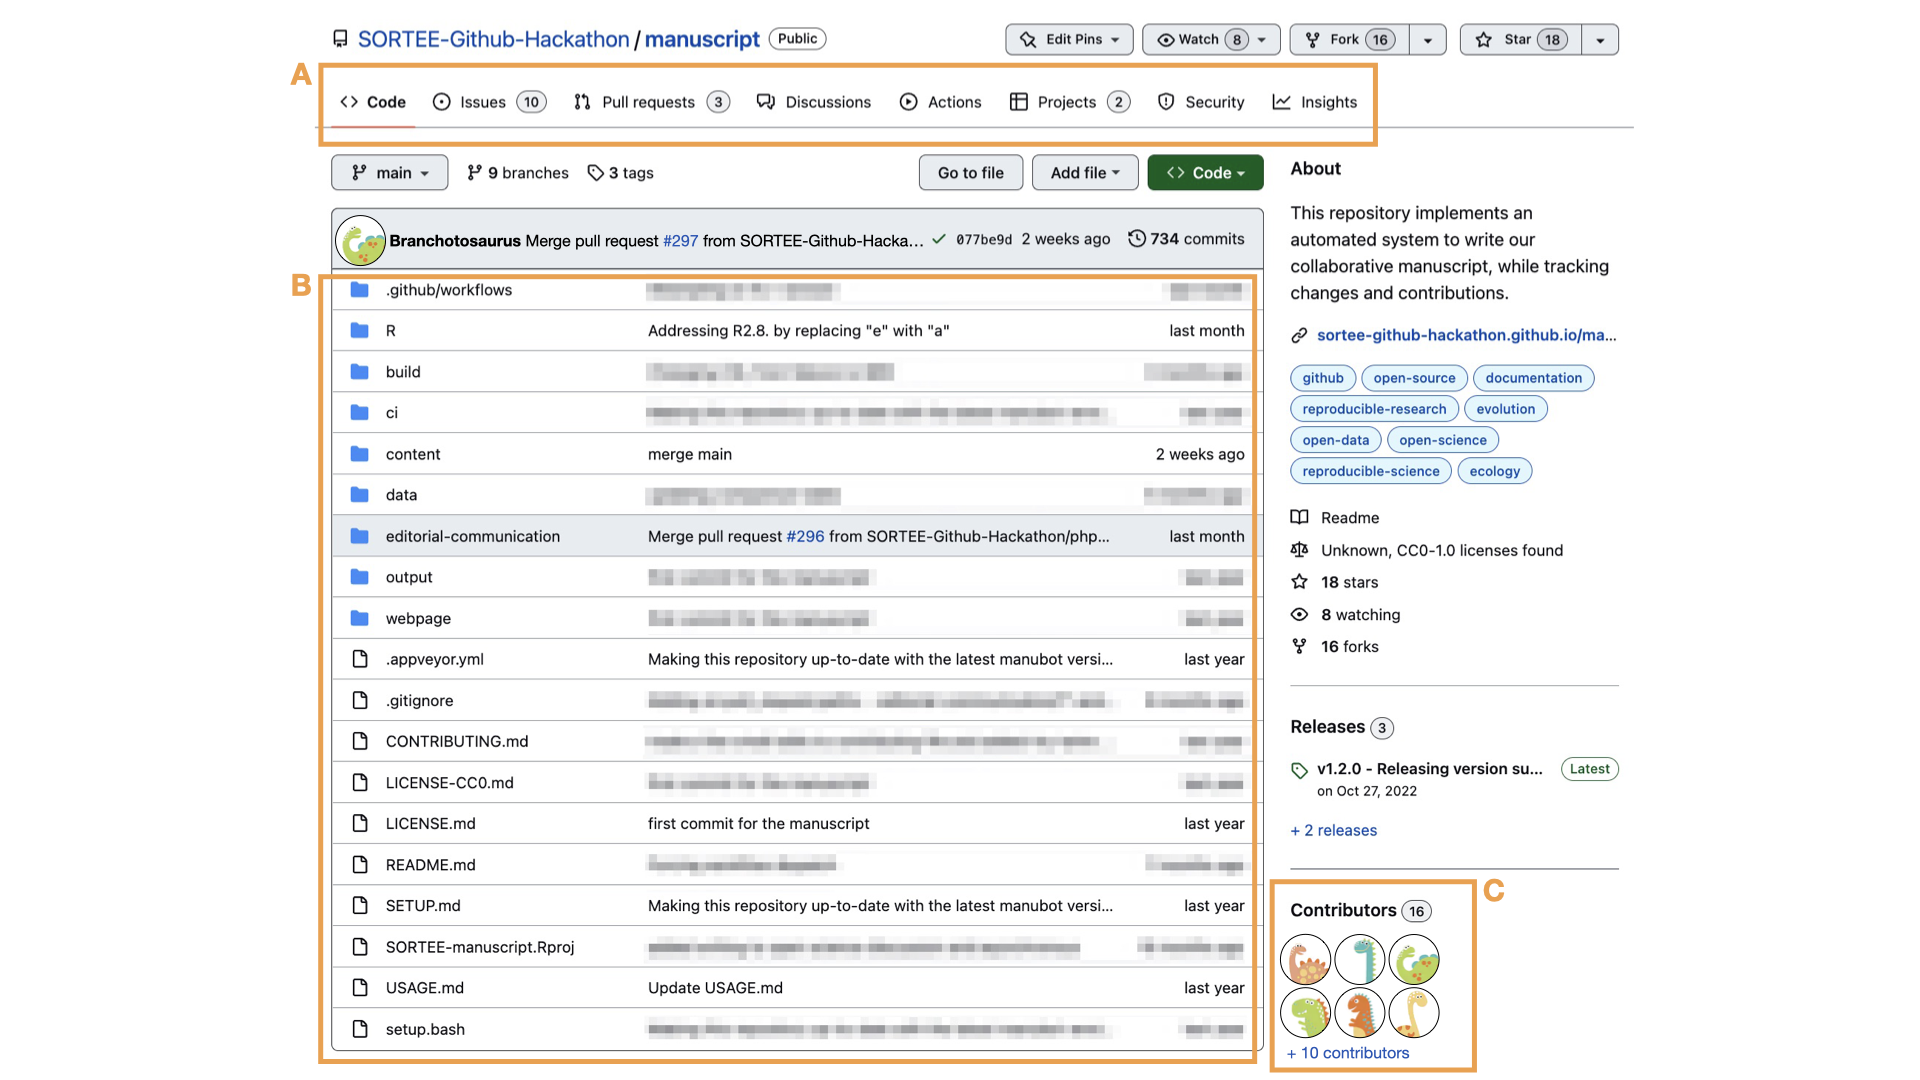
\includegraphics{images/Figure1.png}
\caption{An overview of Git's core features. A) Multi-faceted components allow for code writing, small data storage, manuscript writing, and project management to all be done in one place. \texttt{CONTRIBUTING.md}, \texttt{LICENCE.md}, and \texttt{README.md} files allow new team members, or others wanting to use materials, to understand the project components and learn how they can engage with the project and existing team members. B) Issues, Pull Requests, Discussions, and Projects allow for team members to ask for feedback, suggest fixes, discuss related ideas, and keep track of all the moving parts of a project. C) All collaborators on a project can be a part of a single repository, with varying push privileges and responsibilities.}\label{fig:github-diagram}
}
\end{figure}

\begin{figure}
\hypertarget{fig:scatterblob}{%
\centering
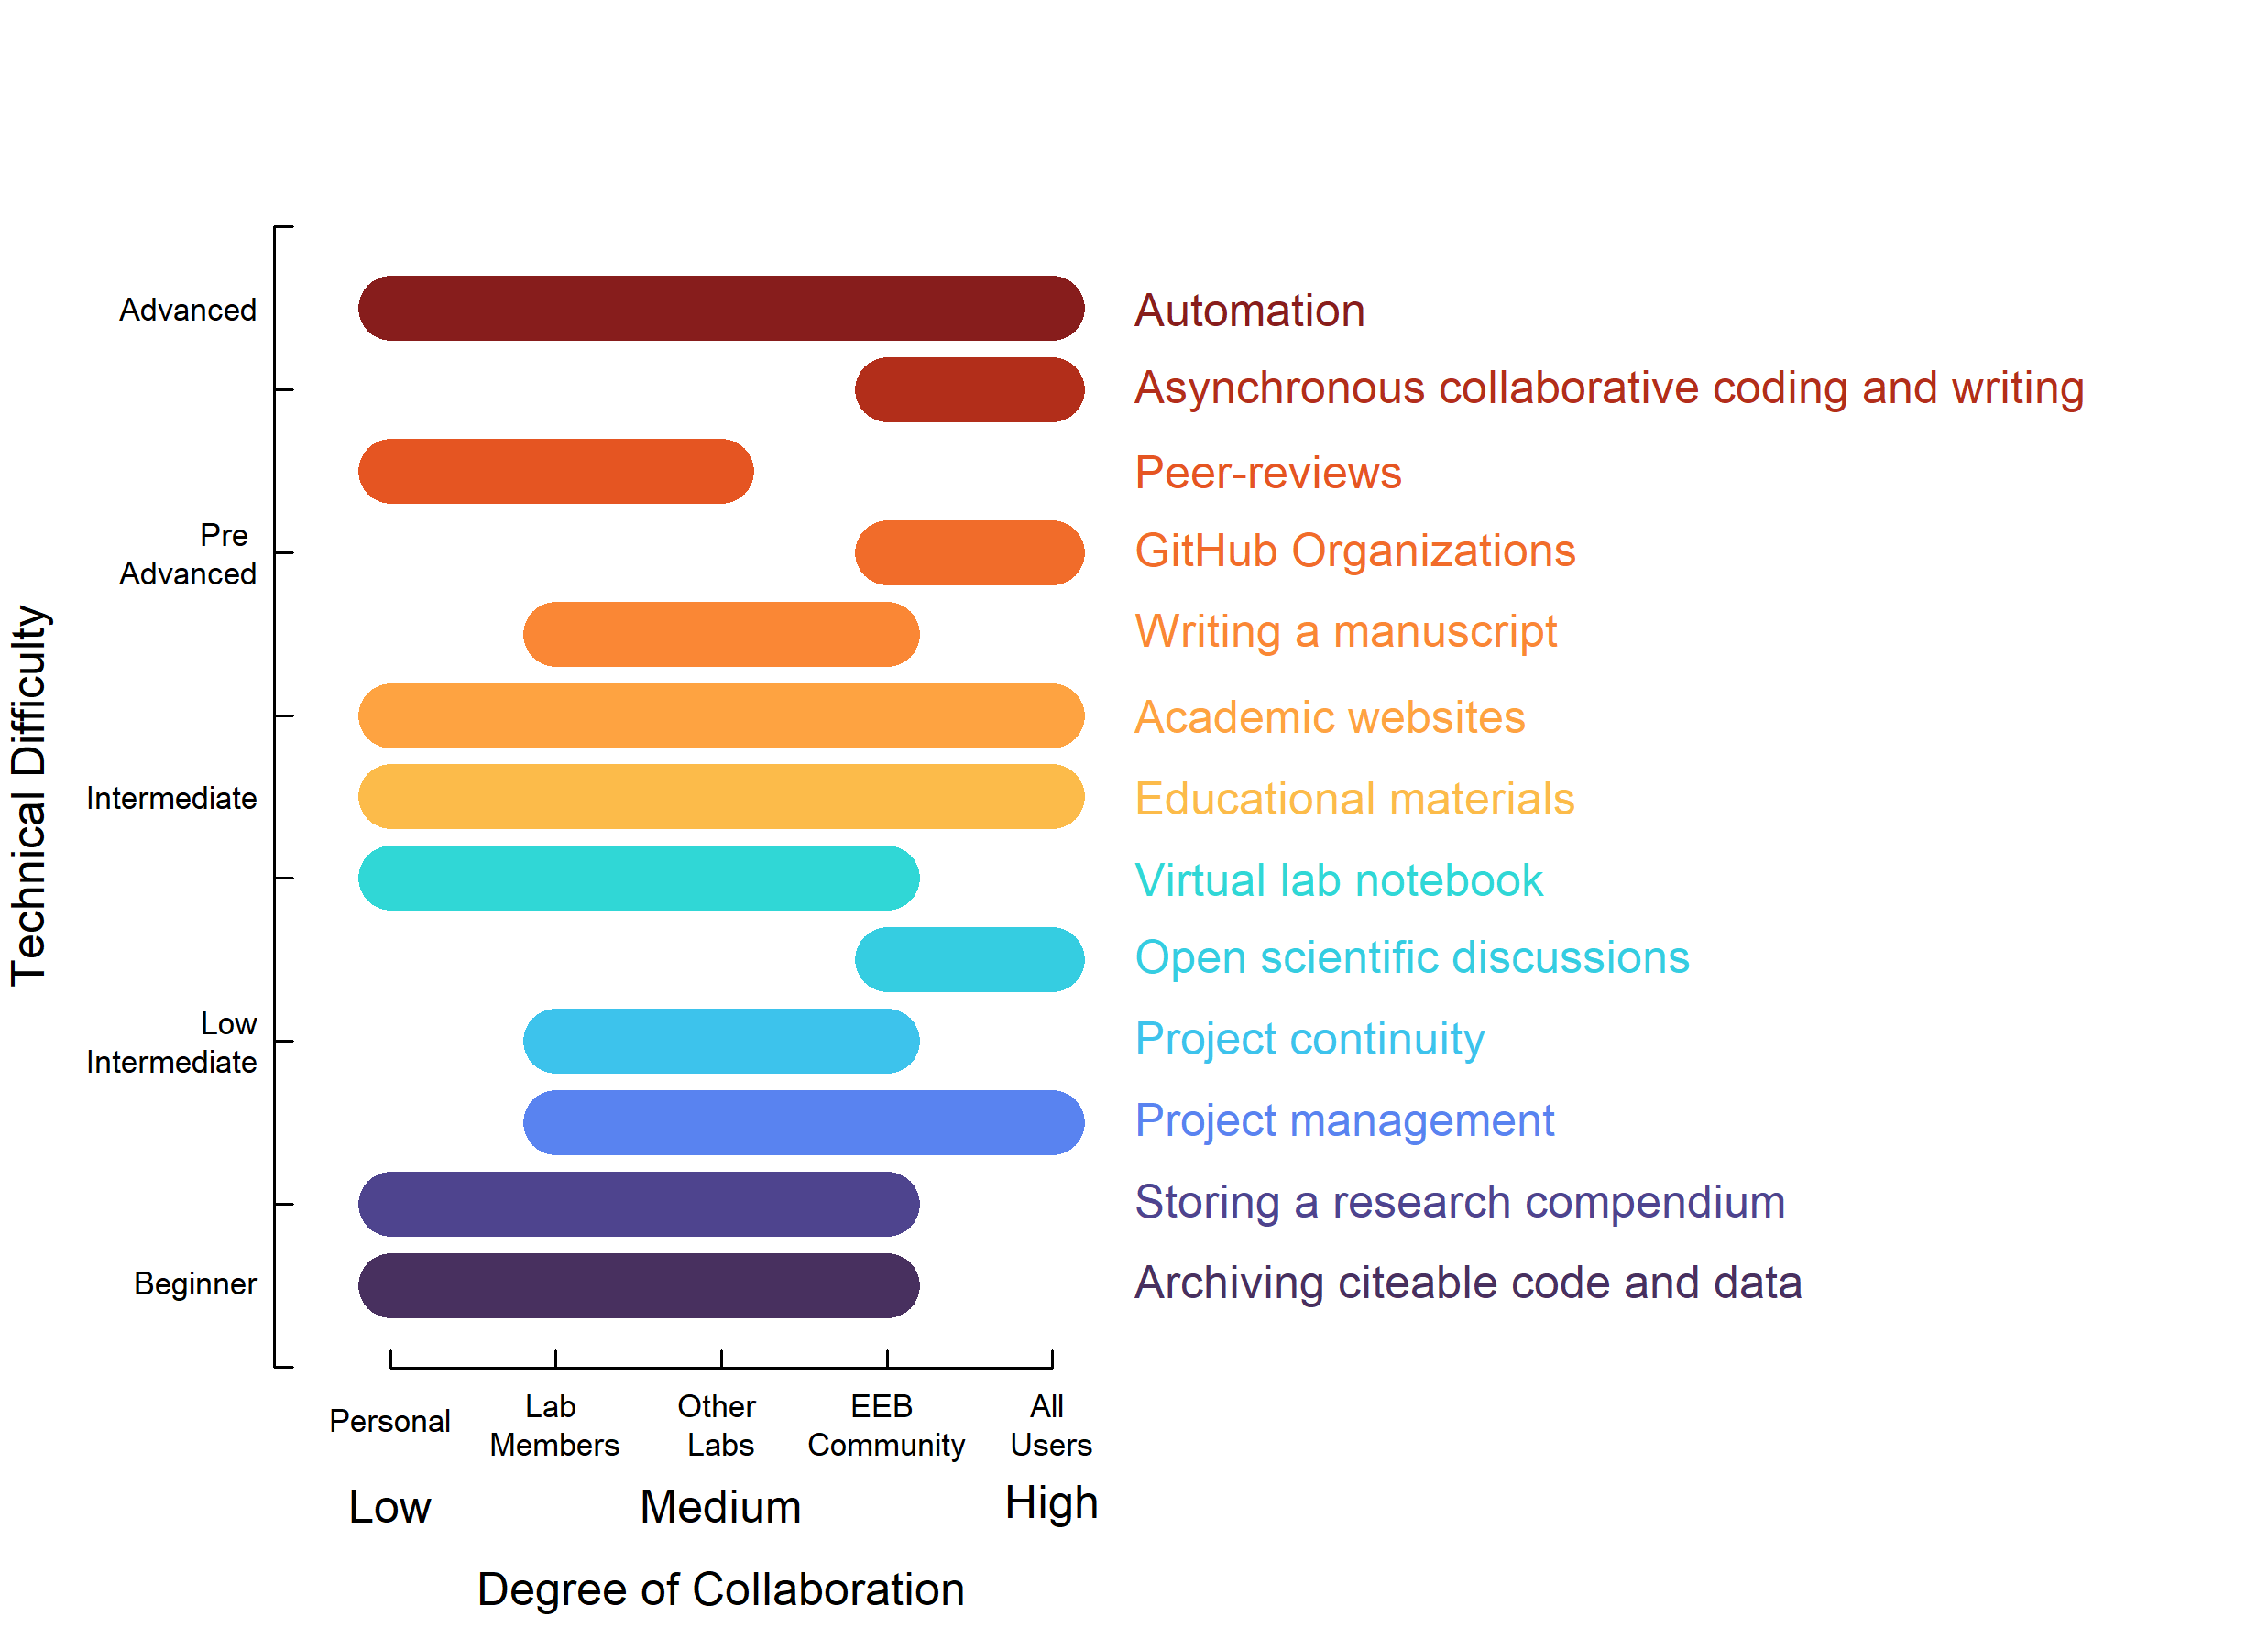
\includegraphics{images/scatterblob_1-viridis-turbo.png}
\caption{A summary of ways GitHub can be used showing technical difficulty and degree of collaboration for each. Activities higher on the vertical axis require usage knowledge of more GitHub features than activities lower on the axis. On the horizontal axis, each activity spans a region representing who is potentially involved with or benefits from each activity. For example, storing data and code mainly benefits individual researchers or members of a laboratory while making data and code citable and reproducible benefit other labs and the larger community as well. Independently of ones knowledge of GitHub features, there are ways to use GitHub that allow tapping unto one of the strongest benefits of the platform: facilitating and enhancing collaboration. For information on the methods and the data used to create this figure, see Appendix S1.1, Appendix S1.2, and Tables S1.1 and S1.2.}\label{fig:scatterblob}
}
\end{figure}

\hypertarget{tables}{%
\subsection{Tables}\label{tables}}

\begin{longtable}[]{@{}
  >{\raggedright\arraybackslash}p{(\columnwidth - 18\tabcolsep) * \real{0.0627}}
  >{\raggedright\arraybackslash}p{(\columnwidth - 18\tabcolsep) * \real{0.0528}}
  >{\raggedright\arraybackslash}p{(\columnwidth - 18\tabcolsep) * \real{0.0281}}
  >{\raggedright\arraybackslash}p{(\columnwidth - 18\tabcolsep) * \real{0.0281}}
  >{\raggedright\arraybackslash}p{(\columnwidth - 18\tabcolsep) * \real{0.0380}}
  >{\raggedright\arraybackslash}p{(\columnwidth - 18\tabcolsep) * \real{0.0528}}
  >{\raggedright\arraybackslash}p{(\columnwidth - 18\tabcolsep) * \real{0.1799}}
  >{\raggedright\arraybackslash}p{(\columnwidth - 18\tabcolsep) * \real{0.1683}}
  >{\raggedright\arraybackslash}p{(\columnwidth - 18\tabcolsep) * \real{0.2558}}
  >{\raggedright\arraybackslash}p{(\columnwidth - 18\tabcolsep) * \real{0.1337}}@{}}
\caption{A comparison of technologies commonly used for collaborating on research in Ecology and Evolutionary Biology. In the first column, we group platforms for collaboration into broad guilds. The second column lists the platform for collaboration. The remaining columns indicate whether the platform for collaboration includes certain features. \label{tbl:compare}}\tabularnewline
\toprule
\begin{minipage}[b]{\linewidth}\raggedright
Guild
\end{minipage} & \begin{minipage}[b]{\linewidth}\raggedright
Software
\end{minipage} & \begin{minipage}[b]{\linewidth}\raggedright
Version control
\end{minipage} & \begin{minipage}[b]{\linewidth}\raggedright
Backup (cloud)
\end{minipage} & \begin{minipage}[b]{\linewidth}\raggedright
Passive collaboration
\end{minipage} & \begin{minipage}[b]{\linewidth}\raggedright
Active real-time collaboration
\end{minipage} & \begin{minipage}[b]{\linewidth}\raggedright
Free plan available
\end{minipage} & \begin{minipage}[b]{\linewidth}\raggedright
Permanent (DOI)
\end{minipage} & \begin{minipage}[b]{\linewidth}\raggedright
Storage limits
\end{minipage} & \begin{minipage}[b]{\linewidth}\raggedright
GitHub Integration
\end{minipage} \\
\midrule
\endfirsthead
\toprule
\begin{minipage}[b]{\linewidth}\raggedright
Guild
\end{minipage} & \begin{minipage}[b]{\linewidth}\raggedright
Software
\end{minipage} & \begin{minipage}[b]{\linewidth}\raggedright
Version control
\end{minipage} & \begin{minipage}[b]{\linewidth}\raggedright
Backup (cloud)
\end{minipage} & \begin{minipage}[b]{\linewidth}\raggedright
Passive collaboration
\end{minipage} & \begin{minipage}[b]{\linewidth}\raggedright
Active real-time collaboration
\end{minipage} & \begin{minipage}[b]{\linewidth}\raggedright
Free plan available
\end{minipage} & \begin{minipage}[b]{\linewidth}\raggedright
Permanent (DOI)
\end{minipage} & \begin{minipage}[b]{\linewidth}\raggedright
Storage limits
\end{minipage} & \begin{minipage}[b]{\linewidth}\raggedright
GitHub Integration
\end{minipage} \\
\midrule
\endhead
Multi-tool & GitHub & yes & yes & yes & no & Broadly used free version. Advanced features are provided for free to students and education professionals. & A DOI can only be obtained when integrating to other services that can mint DOI (e.g., Zenodo, OSF). & 100MB per file, 500MB per private repository (2GB for paid accounts). 100GB for public repositories. Larger files (up to 2GB) can be attached to releases & N/A \\
Multi-tool & Open Science Framework & yes & yes & yes & yes & yes & yes & 25GB for private projects, up to 5GB per file, plus partner add-ons, 50GB for public projects & yes \\
Long-term (public) data repositories & PANGAEA & yes & yes & yes & no & yes & yes & 10 GB free & no \\
Long-term (public) data repositories & Zenodo & after published & after published & yes & no & yes & yes & 50 GB per dataset & yes \\
Long-term (public) data repositories & Dryad & after published & after published & yes & no & some journals cover cost & yes & 300 GB per publication & Can link to individual files (not entire repository), thus not fully integrated \\
Long-term (public) data repositories & Figshare & yes & yes & yes & no & yes & yes & 20 GB free, up to 5 TB & yes \\
Temporary (personal) drive storage & Google Drive & yes & yes & yes & yes & limited free version \& paid & no & 15GB free, up to 100GB with Google One & yes \\
Temporary (personal) drive storage & Box & limited & yes & yes & yes & no & no & Unlimited total size for subscription & yes \\
Temporary (personal) drive storage & DropBox & limited & yes & yes & yes & limited free version \& paid & no & 2GB free & yes \\
Temporary (personal) drive storage & OneDrive and the Office Suite & yes & yes & yes & yes & limited free version \& paid & no & 5 GB free, up to 1TB paid & yes \\
Collaborative code/text editors & Overleaf (online latex editor) & yes & yes & yes & yes & yes & no & 1MB for individual .tex, 50MB for individual files, unlimited project size & yes \\
Collaborative code/text editors & Jupyter Notebook & yes & ? & yes & with Colab & yes & no & via Binder: no hard limit, but suggests no files \textgreater100MB, can also store on GitHub or Google Colab & yes \\
Collaborative code/text editors & HackMD & yes & yes & yes & yes & limited free version \& paid & no & 3 documents free, private invitee limits & yes \\
\bottomrule
\end{longtable}

\begin{longtable}[]{@{}
  >{\raggedright\arraybackslash}p{(\columnwidth - 14\tabcolsep) * \real{0.0493}}
  >{\raggedright\arraybackslash}p{(\columnwidth - 14\tabcolsep) * \real{0.1425}}
  >{\raggedright\arraybackslash}p{(\columnwidth - 14\tabcolsep) * \real{0.1041}}
  >{\raggedright\arraybackslash}p{(\columnwidth - 14\tabcolsep) * \real{0.1562}}
  >{\raggedright\arraybackslash}p{(\columnwidth - 14\tabcolsep) * \real{0.1096}}
  >{\raggedright\arraybackslash}p{(\columnwidth - 14\tabcolsep) * \real{0.1479}}
  >{\raggedright\arraybackslash}p{(\columnwidth - 14\tabcolsep) * \real{0.1370}}
  >{\raggedright\arraybackslash}p{(\columnwidth - 14\tabcolsep) * \real{0.1534}}@{}}
\caption{A non-exhaustive collection of ideas for how various GitHub
features could be utilized for a research project. Here we have
categorized contributors/collaborators into five roles. A Project
Manager owns the GitHub repository for a project, and leads the academic
project (e.g., lead author of a manuscript). A co-author contributes to
writing and other aspects of research, but may have limited or no
experience with programming, git, and/or GitHub. A code contributor
writes or edits analysis code for the project. A code reviewer could be
a project collaborator or a peer reviewer who reviews project code. They
are familiar with coding, but not necessarily with git or GitHub (but
they are willing to learn). Finally, community members could be other
researchers or non-researchers interested in reproducing results,
re-using code or data, or communicating with researchers involved in the
project. These roles are not mutually exclusive---a co-author could also
be a code contributor and code reviewer, for example. For definitions of
the GitHub features, see Box 1. \label{tbl:roles}}\tabularnewline
\toprule
\begin{minipage}[b]{\linewidth}\raggedright
Role
\end{minipage} & \begin{minipage}[b]{\linewidth}\raggedright
GitHub repository
\end{minipage} & \begin{minipage}[b]{\linewidth}\raggedright
README
\end{minipage} & \begin{minipage}[b]{\linewidth}\raggedright
Issue
\end{minipage} & \begin{minipage}[b]{\linewidth}\raggedright
Discussion
\end{minipage} & \begin{minipage}[b]{\linewidth}\raggedright
Pull Request
\end{minipage} & \begin{minipage}[b]{\linewidth}\raggedright
Fork
\end{minipage} & \begin{minipage}[b]{\linewidth}\raggedright
GitHub Pages
\end{minipage} \\
\midrule
\endfirsthead
\toprule
\begin{minipage}[b]{\linewidth}\raggedright
Role
\end{minipage} & \begin{minipage}[b]{\linewidth}\raggedright
GitHub repository
\end{minipage} & \begin{minipage}[b]{\linewidth}\raggedright
README
\end{minipage} & \begin{minipage}[b]{\linewidth}\raggedright
Issue
\end{minipage} & \begin{minipage}[b]{\linewidth}\raggedright
Discussion
\end{minipage} & \begin{minipage}[b]{\linewidth}\raggedright
Pull Request
\end{minipage} & \begin{minipage}[b]{\linewidth}\raggedright
Fork
\end{minipage} & \begin{minipage}[b]{\linewidth}\raggedright
GitHub Pages
\end{minipage} \\
\midrule
\endhead
Project manager & Set contributor permissions, share code of conduct & Project description, citation, DOIs & Assign tasks to collaborators & Discuss project directions and goals & Approve and incorporate edits to code and/or writing & & Share up-to-date reports, figures, or draft manuscript \\
Co-author & Edit Markdown text or add files & & Propose changes involving code (e.g.~analyses, figures) & Discuss proposed changes to manuscript & & & \\
Code contributor & & & Suggest code changes & & Contribute changes to code, initiate code review & & Contribute to project website \\
Code reviewer & Find all code related to a project & & Highlight specific lines of code and make suggestions & & Review or recommended changes in code & & \\
Community & & & Suggest additional features and report bugs & Ask questions about data and code & & Create a linked, editable copy of the repository & View project website \\
\bottomrule
\end{longtable}

\hypertarget{references}{%
\subsection{References}\label{references}}

\hypertarget{refs}{}
\begin{CSLReferences}{1}{0}
\leavevmode\vadjust pre{\hypertarget{ref-s91uGRZ2}{}}%
\emph{About code owners}. (n.d.). GitHub Docs. Retrieved March 4, 2023, from \url{https://ghdocs-prod.azurewebsites.net/en/repositories/managing-your-repositorys-settings-and-features/customizing-your-repository/about-code-owners}

\leavevmode\vadjust pre{\hypertarget{ref-1Co6ZZjF1}{}}%
\emph{About large files on GitHub}. (n.d.). GitHub Docs. Retrieved March 4, 2023, from \url{https://ghdocs-prod.azurewebsites.net/en/repositories/working-with-files/managing-large-files/about-large-files-on-github}

\leavevmode\vadjust pre{\hypertarget{ref-RhBKe0MG}{}}%
\emph{About Projects}. (n.d.). GitHub Docs. Retrieved March 4, 2023, from \url{https://ghdocs-prod.azurewebsites.net/en/issues/planning-and-tracking-with-projects/learning-about-projects/about-projects}

\leavevmode\vadjust pre{\hypertarget{ref-13QX8XU3J}{}}%
Alston, J. M., \& Rick, J. A. (2021). A Beginner's Guide to Conducting Reproducible Research. \emph{The Bulletin of the Ecological Society of America}, \emph{102}(2). \url{https://doi.org/10.1002/bes2.1801}

\leavevmode\vadjust pre{\hypertarget{ref-UsTxAq4f}{}}%
Anbaroğlu, B. (2021). A collaborative GIS programming course using GitHub Classroom. \emph{Transactions in GIS}, \emph{25}(6), 3132--3158. \url{https://doi.org/10.1111/tgis.12810}

\leavevmode\vadjust pre{\hypertarget{ref-PlcxShQU}{}}%
Blischak, J. D., Davenport, E. R., \& Wilson, G. (2016). A Quick Introduction to Version Control with Git and GitHub. \emph{PLOS Computational Biology}, \emph{12}(1), e1004668. \url{https://doi.org/10.1371/journal.pcbi.1004668}

\leavevmode\vadjust pre{\hypertarget{ref-gLby7jt1}{}}%
Borghi, J., \& Van Gulick, A. (2022). Promoting Open Science Through Research Data Management. \emph{Harvard Data Science Review}. \url{https://doi.org/10.1162/99608f92.9497f68e}

\leavevmode\vadjust pre{\hypertarget{ref-ydrk01SR}{}}%
Briney, K., Coates, H., \& Goben, A. (2020). Foundational Practices of Research Data Management. \emph{Research Ideas and Outcomes}, \emph{6}. \url{https://doi.org/10.3897/rio.6.e56508}

\leavevmode\vadjust pre{\hypertarget{ref-RVetqmsg}{}}%
Bryan, J. (2018). Excuse Me, Do You Have a Moment to Talk About Version Control? \emph{The American Statistician}, \emph{72}(1), 20--27. \url{https://doi.org/10.1080/00031305.2017.1399928}

\leavevmode\vadjust pre{\hypertarget{ref-6CMMeSeD}{}}%
Bryan, J., \& TAs, T. S. 545. (n.d.). \emph{STAT 545}. Retrieved March 4, 2023, from \url{https://stat545.com/}

\leavevmode\vadjust pre{\hypertarget{ref-lx49NGto}{}}%
\emph{Connect GitHub to a Project - OSF Support}. (n.d.). Retrieved March 4, 2023, from \url{https://help.osf.io/article/211-connect-github-to-a-project}

\leavevmode\vadjust pre{\hypertarget{ref-1Du6fzB8g}{}}%
Crystal‐Ornelas, R., Varadharajan, C., Bond‐Lamberty, B., Boye, K., Burrus, M., Cholia, S., Crow, M., Damerow, J., Devarakonda, R., Ely, K. S., Goldman, A., Heinz, S., Hendrix, V., Kakalia, Z., Pennington, S. C., Robles, E., Rogers, A., Simmonds, M., Velliquette, T., \ldots{} Agarwal, D. A. (2021). A Guide to Using GitHub for Developing and Versioning Data Standards and Reporting Formats. \emph{Earth and Space Science}, \emph{8}(8). \url{https://doi.org/10.1029/2021ea001797}

\leavevmode\vadjust pre{\hypertarget{ref-D4C4k4ak}{}}%
Fehr, J., Himpe, C., Rave, S., \& Saak, J. (2021). Sustainable Research Software Hand-Over. \emph{Journal of Open Research Software}, \emph{9}(1), 5. \url{https://doi.org/10.5334/jors.307}

\leavevmode\vadjust pre{\hypertarget{ref-1CM2EcdVk}{}}%
\emph{Git - A Short History of Git}. (n.d.). Retrieved March 4, 2023, from \url{https://git-scm.com/book/en/v2/Getting-Started-A-Short-History-of-Git}

\leavevmode\vadjust pre{\hypertarget{ref-VDJput1V}{}}%
Gomes, D. G. E., Pottier, P., Crystal-Ornelas, R., Hudgins, E. J., Foroughirad, V., Sánchez-Reyes, L. L., Turba, R., Martinez, P. A., Moreau, D., Bertram, M. G., Smout, C. A., \& Gaynor, K. M. (2022). Why don't we share data and code? Perceived barriers and benefits to public archiving practices. \emph{Proceedings of the Royal Society B: Biological Sciences}, \emph{289}(1987). \url{https://doi.org/10.1098/rspb.2022.1113}

\leavevmode\vadjust pre{\hypertarget{ref-1HhzKAC1K}{}}%
Goring, S. J., Weathers, K. C., Dodds, W. K., Soranno, P. A., Sweet, L. C., Cheruvelil, K. S., Kominoski, J. S., Rüegg, J., Thorn, A. M., \& Utz, R. M. (2014). Improving the culture of interdisciplinary collaboration in ecology by expanding measures of success. \emph{Frontiers in Ecology and the Environment}, \emph{12}(1), 39--47. \url{https://doi.org/10.1890/120370}

\leavevmode\vadjust pre{\hypertarget{ref-iIEKCTLU}{}}%
Hampton, S. E., Anderson, S. S., Bagby, S. C., Gries, C., Han, X., Hart, E. M., Jones, M. B., Lenhardt, W. C., MacDonald, A., Michener, W. K., Mudge, J., Pourmokhtarian, A., Schildhauer, M. P., Woo, K. H., \& Zimmerman, N. (2015). The Tao of open science for ecology. \emph{Ecosphere}, \emph{6}(7), art120. \url{https://doi.org/10.1890/es14-00402.1}

\leavevmode\vadjust pre{\hypertarget{ref-fJWFe93e}{}}%
Hannay, J. E., MacLeod, C., Singer, J., Langtangen, H. P., Pfahl, D., \& Wilson, G. (2009, May). How do scientists develop and use scientific software? \emph{2009 ICSE Workshop on Software Engineering for Computational Science and Engineering}. 2009 ICSE Workshop on Software Engineering for Computational Science and Engineering (SECSE). \url{https://doi.org/10.1109/secse.2009.5069155}

\leavevmode\vadjust pre{\hypertarget{ref-ZvrOcg9w}{}}%
Hester, J. B., the STAT 545 TAs, Jim. (n.d.). \emph{Let's Git started \textbar{} Happy Git and GitHub for the useR}. Retrieved March 4, 2023, from \url{https://happygitwithr.com/}

\leavevmode\vadjust pre{\hypertarget{ref-3UAritXO}{}}%
\emph{Issues · fmsabatini/sPlotOpen\_Manuscript}. (n.d.). GitHub. Retrieved March 4, 2023, from \url{https://github.com/fmsabatini/sPlotOpen_Manuscript}

\leavevmode\vadjust pre{\hypertarget{ref-ndfO9H}{}}%
Kalliamvakou, E., Damian, D., Blincoe, K., Singer, L., \& German, D. M. (2015, May). Open Source-Style Collaborative Development Practices in Commercial Projects Using GitHub. \emph{2015 IEEE/ACM 37th IEEE International Conference on Software Engineering}. 2015 IEEE/ACM 37th IEEE International Conference on Software Engineering (ICSE). \url{https://doi.org/10.1109/icse.2015.74}

\leavevmode\vadjust pre{\hypertarget{ref-cW7vGddM}{}}%
Khelifa, R., Amano, T., \& Nuñez, M. A. (2022). A solution for breaking the language barrier. \emph{Trends in Ecology \&Amp; Evolution}, \emph{37}(2), 109--112. \url{https://doi.org/10.1016/j.tree.2021.11.003}

\leavevmode\vadjust pre{\hypertarget{ref-lJAgyhYq}{}}%
Kim, A. Y., Herrmann, V., Barreto, R., Calkins, B., Gonzalez‐Akre, E., Johnson, D. J., Jordan, J. A., Magee, L., McGregor, I. R., Montero, N., Novak, K., Rogers, T., Shue, J., \& Anderson‐Teixeira, K. J. (2022). Implementing GitHub Actions continuous integration to reduce error rates in ecological data collection. \emph{Methods in Ecology and Evolution}, \emph{13}(11), 2572--2585. \url{https://doi.org/10.1111/2041-210x.13982}

\leavevmode\vadjust pre{\hypertarget{ref-139b0pSGc}{}}%
Leibzon, W. (2016, August). Social network of software development at GitHub. \emph{2016 IEEE/ACM International Conference on Advances in Social Networks Analysis and Mining (ASONAM)}. 2016 IEEE/ACM International Conference on Advances in Social Networks Analysis and Mining (ASONAM). \url{https://doi.org/10.1109/asonam.2016.7752419}

\leavevmode\vadjust pre{\hypertarget{ref-3DKwn1sY}{}}%
Lowndes, J. S. S., Best, B. D., Scarborough, C., Afflerbach, J. C., Frazier, M. R., O'Hara, C. C., Jiang, N., \& Halpern, B. S. (2017). Our path to better science in less time using open data science tools. \emph{Nature Ecology \&Amp; Evolution}, \emph{1}(6). \url{https://doi.org/10.1038/s41559-017-0160}

\leavevmode\vadjust pre{\hypertarget{ref-pjy75gHr}{}}%
Madicken Munk, Koziar, K., Leinweber, K., Raniere Silva, Michonneau, F., McCue, R., Hejazi, N., Waldman, S., Emonet, R., Harris, R. M., Olex, A. L., Becker, E. A., Lever, J., Burle, M.-H., Moore, B., Umihiko Hoshijima, Maji, A., Topçuoğlu, B. D., Junghans, C., \ldots{} Wolmar Nyberg Åkerström. (2019). \emph{swcarpentry/git-novice: Software Carpentry: Version Control with Git, June 2019} (Version v2019.06.1). Zenodo. \url{https://doi.org/10.5281/zenodo.3264950}

\leavevmode\vadjust pre{\hypertarget{ref-MwwMapRG}{}}%
Marwick, B., Boettiger, C., \& Mullen, L. (2018). Packaging Data Analytical Work Reproducibly Using R (and Friends). \emph{The American Statistician}, \emph{72}(1), 80--88. \url{https://doi.org/10.1080/00031305.2017.1375986}

\leavevmode\vadjust pre{\hypertarget{ref-kEX5dgzK}{}}%
Perez-Riverol, Y., Gatto, L., Wang, R., Sachsenberg, T., Uszkoreit, J., Leprevost, F. da V., Fufezan, C., Ternent, T., Eglen, S. J., Katz, D. S., Pollard, T. J., Konovalov, A., Flight, R. M., Blin, K., \& Vizcaíno, J. A. (2016). Ten Simple Rules for Taking Advantage of Git and GitHub. \emph{PLOS Computational Biology}, \emph{12}(7), e1004947. \url{https://doi.org/10.1371/journal.pcbi.1004947}

\leavevmode\vadjust pre{\hypertarget{ref-10ghgV3S8}{}}%
Perkel, J. (2016). Democratic databases: science on GitHub. \emph{Nature}, \emph{538}(7623), 127--128. \url{https://doi.org/10.1038/538127a}

\leavevmode\vadjust pre{\hypertarget{ref-1Kqna6l2}{}}%
Perkel, J. M. (2020). Challenge to scientists: does your ten-year-old code still run? \emph{Nature}, \emph{584}(7822), 656--658. \url{https://doi.org/10.1038/d41586-020-02462-7}

\leavevmode\vadjust pre{\hypertarget{ref-4ny1onB0}{}}%
Ram, K. (2013). Git can facilitate greater reproducibility and increased transparency in science. \emph{Source Code for Biology and Medicine}, \emph{8}(1). \url{https://doi.org/10.1186/1751-0473-8-7}

\leavevmode\vadjust pre{\hypertarget{ref-HiIPSSHV}{}}%
Smaglik, P. (2007). Creating better lab websites gives potential collaborators and recruiters a clearer window into your world. \emph{Nature}, \emph{447}(7142), 347--347. \url{https://doi.org/10.1038/nj7142-347a}

\leavevmode\vadjust pre{\hypertarget{ref-7q3wZN6d}{}}%
Spinellis, D. (2012). Git. \emph{IEEE Software}, \emph{29}(3), 100--101. \url{https://doi.org/10.1109/ms.2012.61}

\leavevmode\vadjust pre{\hypertarget{ref-dqrFjoSb}{}}%
Trujillo, G., \& Tanner, K. D. (2014). Considering the Role of Affect in Learning: Monitoring Students' Self-Efficacy, Sense of Belonging, and Science Identity. \emph{CBE---Life Sciences Education}, \emph{13}(1), 6--15. \url{https://doi.org/10.1187/cbe.13-12-0241}

\leavevmode\vadjust pre{\hypertarget{ref-19kmNxiHc}{}}%
Vines, Timothy~H., Albert, Arianne~Y. K., Andrew, Rose~L., Débarre, F., Bock, Dan~G., Franklin, Michelle~T., Gilbert, Kimberly~J., Moore, J.-S., Renaut, S., \& Rennison, Diana~J. (2014). The Availability of Research Data Declines Rapidly with Article Age. \emph{Current Biology}, \emph{24}(1), 94--97. \url{https://doi.org/10.1016/j.cub.2013.11.014}

\end{CSLReferences}
